% Options for packages loaded elsewhere
\PassOptionsToPackage{unicode}{hyperref}
\PassOptionsToPackage{hyphens}{url}
\PassOptionsToPackage{dvipsnames,svgnames,x11names}{xcolor}
%
\documentclass[
  letterpaper,
  DIV=11,
  numbers=noendperiod]{scrartcl}

\usepackage{amsmath,amssymb}
\usepackage{iftex}
\ifPDFTeX
  \usepackage[T1]{fontenc}
  \usepackage[utf8]{inputenc}
  \usepackage{textcomp} % provide euro and other symbols
\else % if luatex or xetex
  \usepackage{unicode-math}
  \defaultfontfeatures{Scale=MatchLowercase}
  \defaultfontfeatures[\rmfamily]{Ligatures=TeX,Scale=1}
\fi
\usepackage{lmodern}
\ifPDFTeX\else  
    % xetex/luatex font selection
\fi
% Use upquote if available, for straight quotes in verbatim environments
\IfFileExists{upquote.sty}{\usepackage{upquote}}{}
\IfFileExists{microtype.sty}{% use microtype if available
  \usepackage[]{microtype}
  \UseMicrotypeSet[protrusion]{basicmath} % disable protrusion for tt fonts
}{}
\makeatletter
\@ifundefined{KOMAClassName}{% if non-KOMA class
  \IfFileExists{parskip.sty}{%
    \usepackage{parskip}
  }{% else
    \setlength{\parindent}{0pt}
    \setlength{\parskip}{6pt plus 2pt minus 1pt}}
}{% if KOMA class
  \KOMAoptions{parskip=half}}
\makeatother
\usepackage{xcolor}
\setlength{\emergencystretch}{3em} % prevent overfull lines
\setcounter{secnumdepth}{-\maxdimen} % remove section numbering
% Make \paragraph and \subparagraph free-standing
\makeatletter
\ifx\paragraph\undefined\else
  \let\oldparagraph\paragraph
  \renewcommand{\paragraph}{
    \@ifstar
      \xxxParagraphStar
      \xxxParagraphNoStar
  }
  \newcommand{\xxxParagraphStar}[1]{\oldparagraph*{#1}\mbox{}}
  \newcommand{\xxxParagraphNoStar}[1]{\oldparagraph{#1}\mbox{}}
\fi
\ifx\subparagraph\undefined\else
  \let\oldsubparagraph\subparagraph
  \renewcommand{\subparagraph}{
    \@ifstar
      \xxxSubParagraphStar
      \xxxSubParagraphNoStar
  }
  \newcommand{\xxxSubParagraphStar}[1]{\oldsubparagraph*{#1}\mbox{}}
  \newcommand{\xxxSubParagraphNoStar}[1]{\oldsubparagraph{#1}\mbox{}}
\fi
\makeatother

\usepackage{color}
\usepackage{fancyvrb}
\newcommand{\VerbBar}{|}
\newcommand{\VERB}{\Verb[commandchars=\\\{\}]}
\DefineVerbatimEnvironment{Highlighting}{Verbatim}{commandchars=\\\{\}}
% Add ',fontsize=\small' for more characters per line
\usepackage{framed}
\definecolor{shadecolor}{RGB}{241,243,245}
\newenvironment{Shaded}{\begin{snugshade}}{\end{snugshade}}
\newcommand{\AlertTok}[1]{\textcolor[rgb]{0.68,0.00,0.00}{#1}}
\newcommand{\AnnotationTok}[1]{\textcolor[rgb]{0.37,0.37,0.37}{#1}}
\newcommand{\AttributeTok}[1]{\textcolor[rgb]{0.40,0.45,0.13}{#1}}
\newcommand{\BaseNTok}[1]{\textcolor[rgb]{0.68,0.00,0.00}{#1}}
\newcommand{\BuiltInTok}[1]{\textcolor[rgb]{0.00,0.23,0.31}{#1}}
\newcommand{\CharTok}[1]{\textcolor[rgb]{0.13,0.47,0.30}{#1}}
\newcommand{\CommentTok}[1]{\textcolor[rgb]{0.37,0.37,0.37}{#1}}
\newcommand{\CommentVarTok}[1]{\textcolor[rgb]{0.37,0.37,0.37}{\textit{#1}}}
\newcommand{\ConstantTok}[1]{\textcolor[rgb]{0.56,0.35,0.01}{#1}}
\newcommand{\ControlFlowTok}[1]{\textcolor[rgb]{0.00,0.23,0.31}{\textbf{#1}}}
\newcommand{\DataTypeTok}[1]{\textcolor[rgb]{0.68,0.00,0.00}{#1}}
\newcommand{\DecValTok}[1]{\textcolor[rgb]{0.68,0.00,0.00}{#1}}
\newcommand{\DocumentationTok}[1]{\textcolor[rgb]{0.37,0.37,0.37}{\textit{#1}}}
\newcommand{\ErrorTok}[1]{\textcolor[rgb]{0.68,0.00,0.00}{#1}}
\newcommand{\ExtensionTok}[1]{\textcolor[rgb]{0.00,0.23,0.31}{#1}}
\newcommand{\FloatTok}[1]{\textcolor[rgb]{0.68,0.00,0.00}{#1}}
\newcommand{\FunctionTok}[1]{\textcolor[rgb]{0.28,0.35,0.67}{#1}}
\newcommand{\ImportTok}[1]{\textcolor[rgb]{0.00,0.46,0.62}{#1}}
\newcommand{\InformationTok}[1]{\textcolor[rgb]{0.37,0.37,0.37}{#1}}
\newcommand{\KeywordTok}[1]{\textcolor[rgb]{0.00,0.23,0.31}{\textbf{#1}}}
\newcommand{\NormalTok}[1]{\textcolor[rgb]{0.00,0.23,0.31}{#1}}
\newcommand{\OperatorTok}[1]{\textcolor[rgb]{0.37,0.37,0.37}{#1}}
\newcommand{\OtherTok}[1]{\textcolor[rgb]{0.00,0.23,0.31}{#1}}
\newcommand{\PreprocessorTok}[1]{\textcolor[rgb]{0.68,0.00,0.00}{#1}}
\newcommand{\RegionMarkerTok}[1]{\textcolor[rgb]{0.00,0.23,0.31}{#1}}
\newcommand{\SpecialCharTok}[1]{\textcolor[rgb]{0.37,0.37,0.37}{#1}}
\newcommand{\SpecialStringTok}[1]{\textcolor[rgb]{0.13,0.47,0.30}{#1}}
\newcommand{\StringTok}[1]{\textcolor[rgb]{0.13,0.47,0.30}{#1}}
\newcommand{\VariableTok}[1]{\textcolor[rgb]{0.07,0.07,0.07}{#1}}
\newcommand{\VerbatimStringTok}[1]{\textcolor[rgb]{0.13,0.47,0.30}{#1}}
\newcommand{\WarningTok}[1]{\textcolor[rgb]{0.37,0.37,0.37}{\textit{#1}}}

\providecommand{\tightlist}{%
  \setlength{\itemsep}{0pt}\setlength{\parskip}{0pt}}\usepackage{longtable,booktabs,array}
\usepackage{calc} % for calculating minipage widths
% Correct order of tables after \paragraph or \subparagraph
\usepackage{etoolbox}
\makeatletter
\patchcmd\longtable{\par}{\if@noskipsec\mbox{}\fi\par}{}{}
\makeatother
% Allow footnotes in longtable head/foot
\IfFileExists{footnotehyper.sty}{\usepackage{footnotehyper}}{\usepackage{footnote}}
\makesavenoteenv{longtable}
\usepackage{graphicx}
\makeatletter
\newsavebox\pandoc@box
\newcommand*\pandocbounded[1]{% scales image to fit in text height/width
  \sbox\pandoc@box{#1}%
  \Gscale@div\@tempa{\textheight}{\dimexpr\ht\pandoc@box+\dp\pandoc@box\relax}%
  \Gscale@div\@tempb{\linewidth}{\wd\pandoc@box}%
  \ifdim\@tempb\p@<\@tempa\p@\let\@tempa\@tempb\fi% select the smaller of both
  \ifdim\@tempa\p@<\p@\scalebox{\@tempa}{\usebox\pandoc@box}%
  \else\usebox{\pandoc@box}%
  \fi%
}
% Set default figure placement to htbp
\def\fps@figure{htbp}
\makeatother

\KOMAoption{captions}{tableheading}
\makeatletter
\@ifpackageloaded{tcolorbox}{}{\usepackage[skins,breakable]{tcolorbox}}
\@ifpackageloaded{fontawesome5}{}{\usepackage{fontawesome5}}
\definecolor{quarto-callout-color}{HTML}{909090}
\definecolor{quarto-callout-note-color}{HTML}{0758E5}
\definecolor{quarto-callout-important-color}{HTML}{CC1914}
\definecolor{quarto-callout-warning-color}{HTML}{EB9113}
\definecolor{quarto-callout-tip-color}{HTML}{00A047}
\definecolor{quarto-callout-caution-color}{HTML}{FC5300}
\definecolor{quarto-callout-color-frame}{HTML}{acacac}
\definecolor{quarto-callout-note-color-frame}{HTML}{4582ec}
\definecolor{quarto-callout-important-color-frame}{HTML}{d9534f}
\definecolor{quarto-callout-warning-color-frame}{HTML}{f0ad4e}
\definecolor{quarto-callout-tip-color-frame}{HTML}{02b875}
\definecolor{quarto-callout-caution-color-frame}{HTML}{fd7e14}
\makeatother
\makeatletter
\@ifpackageloaded{caption}{}{\usepackage{caption}}
\AtBeginDocument{%
\ifdefined\contentsname
  \renewcommand*\contentsname{Table of contents}
\else
  \newcommand\contentsname{Table of contents}
\fi
\ifdefined\listfigurename
  \renewcommand*\listfigurename{List of Figures}
\else
  \newcommand\listfigurename{List of Figures}
\fi
\ifdefined\listtablename
  \renewcommand*\listtablename{List of Tables}
\else
  \newcommand\listtablename{List of Tables}
\fi
\ifdefined\figurename
  \renewcommand*\figurename{Figure}
\else
  \newcommand\figurename{Figure}
\fi
\ifdefined\tablename
  \renewcommand*\tablename{Table}
\else
  \newcommand\tablename{Table}
\fi
}
\@ifpackageloaded{float}{}{\usepackage{float}}
\floatstyle{ruled}
\@ifundefined{c@chapter}{\newfloat{codelisting}{h}{lop}}{\newfloat{codelisting}{h}{lop}[chapter]}
\floatname{codelisting}{Listing}
\newcommand*\listoflistings{\listof{codelisting}{List of Listings}}
\makeatother
\makeatletter
\makeatother
\makeatletter
\@ifpackageloaded{caption}{}{\usepackage{caption}}
\@ifpackageloaded{subcaption}{}{\usepackage{subcaption}}
\makeatother

\usepackage{bookmark}

\IfFileExists{xurl.sty}{\usepackage{xurl}}{} % add URL line breaks if available
\urlstyle{same} % disable monospaced font for URLs
\hypersetup{
  pdftitle={Homework 3},
  pdfauthor={Your name here - update this!!!!},
  colorlinks=true,
  linkcolor={blue},
  filecolor={Maroon},
  citecolor={Blue},
  urlcolor={Blue},
  pdfcreator={LaTeX via pandoc}}


\title{Homework 3}
\usepackage{etoolbox}
\makeatletter
\providecommand{\subtitle}[1]{% add subtitle to \maketitle
  \apptocmd{\@title}{\par {\large #1 \par}}{}{}
}
\makeatother
\subtitle{BSTA 513/613}
\author{Your name here - update this!!!!}
\date{}

\begin{document}
\maketitle


\begin{tcolorbox}[enhanced jigsaw, left=2mm, colback=white, opacityback=0, bottomrule=.15mm, colframe=quarto-callout-caution-color-frame, rightrule=.15mm, breakable, coltitle=black, arc=.35mm, toptitle=1mm, bottomtitle=1mm, opacitybacktitle=0.6, leftrule=.75mm, titlerule=0mm, toprule=.15mm, colbacktitle=quarto-callout-caution-color!10!white, title=\textcolor{quarto-callout-caution-color}{\faFire}\hspace{0.5em}{Caution}]

Homework is ready to go!! (5/5/2025)

\end{tcolorbox}

\subsection{Purpose}\label{purpose}

This homework is designed to help you practice the following important
skills and knowledge that we covered in Lesson 10-12:

\begin{itemize}
\tightlist
\item
  A bunch of work on interactions
\item
  Identifying numerical problems and thinking through potential fixes
\item
  Assessing overall measure of model fit
\end{itemize}

\subsection{Directions}\label{directions}

\begin{itemize}
\item
  \href{https://github.com/nwakim/BSTA_513_S25/blob/main/homework/HW_03.qmd}{Download
  the \texttt{.qmd} file here.}
\item
  You will need to download the datasets from our shared folder.
\item
  Please upload your homework to Sakai. Upload both your .qmd code file
  and the rendered .html file

  \begin{itemize}
  \tightlist
  \item
    Please rename you homework as Lastname\_Firstinitial\_HW02.qmd. This
    will help organize the homeworks when the TAs grade them.
  \end{itemize}
\item
  For each question, make sure to include all code and resulting output
  in the html file to support your answers
\item
  Show the work of your calculations using R code within a code chunk.
  Make sure that both your code and output are visible in the rendered
  html file. This is the default setting.
\end{itemize}

\begin{tcolorbox}[enhanced jigsaw, left=2mm, colback=white, opacityback=0, bottomrule=.15mm, colframe=quarto-callout-tip-color-frame, rightrule=.15mm, breakable, coltitle=black, arc=.35mm, toptitle=1mm, bottomtitle=1mm, opacitybacktitle=0.6, leftrule=.75mm, titlerule=0mm, toprule=.15mm, colbacktitle=quarto-callout-tip-color!10!white, title=\textcolor{quarto-callout-tip-color}{\faLightbulb}\hspace{0.5em}{Tip}]

It is a good idea to try rendering your document from time to time as
you go along! Note that rendering automatically saves your qmd file and
rendering frequently helps you catch your errors more quickly.

\end{tcolorbox}

\subsection{Questions Part 1}\label{questions-part-1}

\subsubsection{Question 1}\label{question-1}

This question is taken from the Hosmer and Lemeshow textbook. The ICU
study data set consists of a sample of 200 subjects who were part of a
much larger study on survival of patients following admission to an
adult intensive care unit (ICU). The dataset should be available in our
shared folder. The major goal of this study was to develop a logistic
regression model to predict the probability of survival to hospital
discharge of these patients. In this question, the primary outcome
variable is vital (survival) status at hospital discharge, STA.
Clinicians associated with the study felt that a key determinant of
survival was the patient's age at admission, AGE. We will build to a
multivariable logistic regression model while adjusting for cancer part
of the present problem (CAN), CPR prior to ICU admission (CPR),
infection probable at ICU admission (INF), and level of consciousness at
ICU admission (LOC).

A code sheet for the variables to be considered is displayed in Table
1.5 below (from the Hosmer and Lemeshow textbook, pg. 23). We refer to
this data set as the ICU data.

\textbf{You will need to use some of the mutations implemented in
\href{https://nwakim.github.io/BSTA_513_S25/homework/HW_02.html\#part-d-1}{HW
2, Q2, Part d}.}

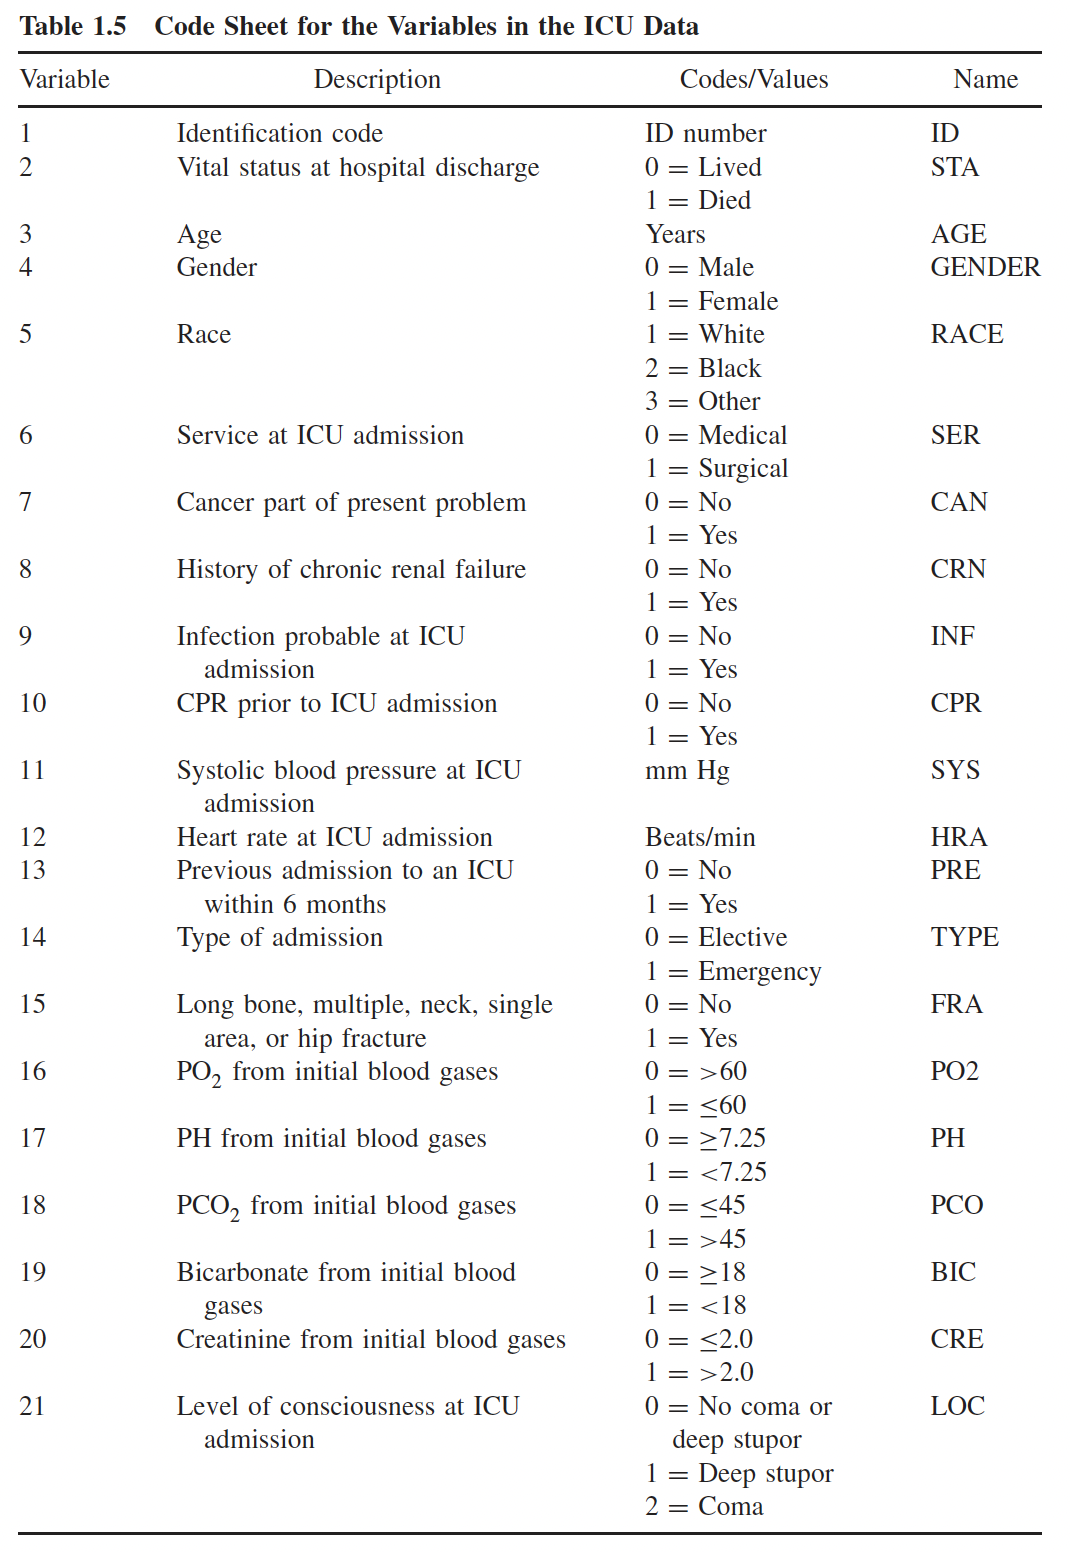
\includegraphics[width=5.80208in,height=\textheight,keepaspectratio]{./images/ICU_codebook.png}

\paragraph{Part a}\label{part-a}

Write down the population equation for the logistic regression model of
STA on AGE, CAN, CPR, and INF. How many parameters does this model
contain?

\paragraph{Part b}\label{part-b}

Using \texttt{glm()}, obtain the maximum likelihood estimates of the
parameters of the logistic regression model in Part a. Using these
estimates, write down the equation with the fitted values.

\paragraph{Part c}\label{part-c}

Assess the significance of the group of coefficients for all variables
in the model using the likelihood ratio test. (Hint: part of the ratio
in the LRT will be an intercept only model)

\paragraph{Part d}\label{part-d}

Fit a new model using only CAN and INF as the predictors, including an
interaction between CAN and INF. Is there evidence that our model should
have an interaction between CAN and INF (Hint: this requires a formal
test of the interaction)?

\paragraph{Part e}\label{part-e}

Interpret the odds ratio for the \textbf{main effects} in the model from
Part d.~Please include the 95\% confidence interval.

\paragraph{Part f}\label{part-f}

From the above model, fill out the following table for the odds ratios.
Note, you will only need to report two odds ratios and you already have
one from Part d \& e.

\begin{longtable}[]{@{}
  >{\raggedright\arraybackslash}p{(\linewidth - 6\tabcolsep) * \real{0.2740}}
  >{\raggedright\arraybackslash}p{(\linewidth - 6\tabcolsep) * \real{0.2603}}
  >{\raggedright\arraybackslash}p{(\linewidth - 6\tabcolsep) * \real{0.2329}}
  >{\raggedright\arraybackslash}p{(\linewidth - 6\tabcolsep) * \real{0.2329}}@{}}
\toprule\noalign{}
\begin{minipage}[b]{\linewidth}\raggedright
Cancer
\end{minipage} & \begin{minipage}[b]{\linewidth}\raggedright
Infection
\end{minipage} & \begin{minipage}[b]{\linewidth}\raggedright
Estimated odds ratio
\end{minipage} & \begin{minipage}[b]{\linewidth}\raggedright
95\% CI
\end{minipage} \\
\midrule\noalign{}
\endhead
\bottomrule\noalign{}
\endlastfoot
Cancer part of present problem & Infection probable at ICU intake & & \\
& ~ ~ ~~No & & \\
& ~ ~ ~~Yes & FILL HERE & FILL HERE \\
Cancer not part of present problem & Infection probable at ICU intake &
& \\
& ~ ~ ~~No & & \\
& ~ ~ ~~Yes & FILL HERE & FILL HERE \\
\end{longtable}

This is a really good way to report odds ratios for interactions between
two categorical predictors! Might want to keep this in mind for your
project!!

\paragraph{Part g}\label{part-g}

Interpret the odds ratio from the table in Part e. Please include the
95\% confidence interval. What do you notice about the odds ratios
(Hint: Think back to my last slides in Lesson 10: Interactions)?

\paragraph{Part h}\label{part-h}

Compute the predicted probability for a subject who does not have a
present issue with cancer nor an infection upon admittance to the ICU.
Compute the 95\% confidence interval for the predicted probability. Can
you use the Normal approximation?

\paragraph{Part i}\label{part-i}

Interpret the predicted probability from Part h (right above), including
the confidence interval.

\paragraph{Part j}\label{part-j}

Building off of Part e, fill out the following table for predicted
probabilities. What do you notice about the predicted probabilities
(Hint: Think back to my last slides in Lesson 10: Interactions)?

\begin{longtable}[]{@{}
  >{\raggedright\arraybackslash}p{(\linewidth - 6\tabcolsep) * \real{0.2603}}
  >{\raggedright\arraybackslash}p{(\linewidth - 6\tabcolsep) * \real{0.2466}}
  >{\raggedright\arraybackslash}p{(\linewidth - 6\tabcolsep) * \real{0.2466}}
  >{\raggedright\arraybackslash}p{(\linewidth - 6\tabcolsep) * \real{0.2466}}@{}}
\toprule\noalign{}
\begin{minipage}[b]{\linewidth}\raggedright
Cancer
\end{minipage} & \begin{minipage}[b]{\linewidth}\raggedright
Infection
\end{minipage} & \begin{minipage}[b]{\linewidth}\raggedright
Predicted probability
\end{minipage} & \begin{minipage}[b]{\linewidth}\raggedright
95\% CI
\end{minipage} \\
\midrule\noalign{}
\endhead
\bottomrule\noalign{}
\endlastfoot
Cancer part of present problem & Infection probable at ICU intake & & \\
& ~ ~ ~~No & FILL HERE & FILL HERE \\
& ~ ~ ~~Yes & FILL HERE & FILL HERE \\
Cancer not part of present problem & Infection probable at ICU intake &
& \\
& ~ ~ ~~No & FILL HERE & FILL HERE \\
& ~ ~ ~~Yes & FILL HERE & FILL HERE \\
\end{longtable}

\subsubsection{Question 2}\label{question-2}

We will continue with the same dataset from Question 1 above.

We will use the model from Question 1a for this question:
\[\text{logit}(\pi(\textbf{X}))=\beta_0 + \beta_1 \cdot AGE + \beta_2 \cdot I(CAN=\text{``Yes"}) + \beta_3 \cdot I(CPR=\text{``Yes"}) + \\ \beta_4 \cdot I(INF=\text{``Yes"})\]

\begin{Shaded}
\begin{Highlighting}[]
\NormalTok{icu }\OtherTok{=} \FunctionTok{read\_csv}\NormalTok{(}\FunctionTok{here}\NormalTok{(}\StringTok{"data"}\NormalTok{, }\StringTok{"icu.csv"}\NormalTok{))}
\NormalTok{icu1 }\OtherTok{=}\NormalTok{ icu }\SpecialCharTok{\%\textgreater{}\%} \FunctionTok{mutate}\NormalTok{(}\AttributeTok{STA =} \FunctionTok{as.factor}\NormalTok{(STA) }\SpecialCharTok{\%\textgreater{}\%} \FunctionTok{relevel}\NormalTok{(}\AttributeTok{ref =} \StringTok{"Lived"}\NormalTok{))}
\NormalTok{icu2 }\OtherTok{=}\NormalTok{ icu1 }\SpecialCharTok{\%\textgreater{}\%} \FunctionTok{mutate}\NormalTok{(}\AttributeTok{CAN =} \FunctionTok{as.factor}\NormalTok{(CAN) }\SpecialCharTok{\%\textgreater{}\%} \FunctionTok{relevel}\NormalTok{(}\AttributeTok{ref =} \StringTok{"No"}\NormalTok{), }
                     \AttributeTok{CPR =} \FunctionTok{as.factor}\NormalTok{(CPR) }\SpecialCharTok{\%\textgreater{}\%} \FunctionTok{relevel}\NormalTok{(}\AttributeTok{ref =} \StringTok{"No"}\NormalTok{), }
                     \AttributeTok{INF =} \FunctionTok{as.factor}\NormalTok{(INF) }\SpecialCharTok{\%\textgreater{}\%} \FunctionTok{relevel}\NormalTok{(}\AttributeTok{ref =} \StringTok{"No"}\NormalTok{), }
                     \AttributeTok{LOC =} \FunctionTok{as.factor}\NormalTok{(LOC) }\SpecialCharTok{\%\textgreater{}\%} 
                       \FunctionTok{relevel}\NormalTok{(}\AttributeTok{ref =} \StringTok{"No Coma or Deep Stupor"}\NormalTok{))}
\end{Highlighting}
\end{Shaded}

\paragraph{Part a}\label{part-a-1}

Assess the fit of the above model. You may use Hosmer-Lemeshow test or
Pearson Residual as appropriate. Discuss your choice and interpret.

\paragraph{Part b}\label{part-b-1}

Assess the your model's ability to discriminate vital status (STA) using
AUC.

\paragraph{Part c}\label{part-c-1}

Let's say a colleague found a different preliminary final model than
yours. Using the below model that your colleague fit, compare your model
to theirs using AIC and BIC.

\[\begin{align} \text{logit}(\pi(\textbf{X})) = & \beta_0 + \beta_1 \cdot AGE + \beta_2 \cdot I(SYS=\text{``Yes"}) + \beta_3 \cdot I(CPR=\text{``Yes"}) + \\ & \beta_4 \cdot I(INF=\text{``Yes"}) + \beta_5 \cdot I(CPR=\text{``Yes"}) \cdot AGE \end{align}\]

\subsubsection{Question 3}\label{question-3}

This question stems from an example from an
\href{https://bookdown.org/rwnahhas/RMPH/}{online textbook} by Dr.~Ramzi
W. Nahhas. The dataset for this problem includes a subset of individuals
from the 2019 National Survey on Drug Use and Health (NSDUH). Overall,
our study aims included investigating potential risk factors for
lifetime heroin use. Lifetime heroin use is a binary outcome, which we
regress on age at first use of alcohol (alc\_agefirst), age with 6
categories (demog\_age\_cat6), and sex assigned at birth (demog\_sex).

\begin{Shaded}
\begin{Highlighting}[]
\FunctionTok{load}\NormalTok{(}\FunctionTok{here}\NormalTok{(}\StringTok{"data"}\NormalTok{, }\StringTok{"nsduh2019\_adult\_sub\_rmph.RData"}\NormalTok{))}
\NormalTok{nsduh }\OtherTok{=}\NormalTok{ nsduh\_adult\_sub }\SpecialCharTok{\%\textgreater{}\%} 
\NormalTok{  dplyr}\SpecialCharTok{::}\FunctionTok{select}\NormalTok{(her\_lifetime, alc\_agefirst, demog\_age\_cat6, demog\_sex) }\SpecialCharTok{\%\textgreater{}\%} 
  \FunctionTok{drop\_na}\NormalTok{()}
\end{Highlighting}
\end{Shaded}

\paragraph{Part a}\label{part-a-2}

Using the \texttt{nsduh} dataset from the above chunk of code, please
run a regression model using lifetime heroin use as our outcome, and age
at first use of alcohol, categorical age, and sex assigned at birth as
covariates in our model. No need to write out your model, you just need
to write the R code to run the regression and display the summary.

\paragraph{Part b}\label{part-b-2}

Are we encountering a numerical problem with our regression? If yes,
please name the numerical issue. What first clued you into that issue?
Provide conclusive evidence of this numerical issue (with a contingency
table), and explain which variable(s) are causing this problem.

\paragraph{Part c}\label{part-c-2}

What would you do to ``fix'' this numerical issue? Please apply your
``fix'' and rerun the regression

\subsection{Questions Part 2}\label{questions-part-2}

The following questions are intended to give you \textbf{practice in
connecting concepts} that will help you make decisions in real world
applications.

\subsubsection{Question 4}\label{question-4}

Using a similar table to the one in Lesson 8, go back through the parts
in this homework and determine which test can be run.

\begin{longtable}[]{@{}
  >{\raggedright\arraybackslash}p{(\linewidth - 6\tabcolsep) * \real{0.2703}}
  >{\raggedright\arraybackslash}p{(\linewidth - 6\tabcolsep) * \real{0.2432}}
  >{\raggedright\arraybackslash}p{(\linewidth - 6\tabcolsep) * \real{0.2432}}
  >{\raggedright\arraybackslash}p{(\linewidth - 6\tabcolsep) * \real{0.2432}}@{}}
\toprule\noalign{}
\begin{minipage}[b]{\linewidth}\raggedright
\end{minipage} & \begin{minipage}[b]{\linewidth}\raggedright
Wald test/CI
\end{minipage} & \begin{minipage}[b]{\linewidth}\raggedright
Score test
\end{minipage} & \begin{minipage}[b]{\linewidth}\raggedright
LRT
\end{minipage} \\
\midrule\noalign{}
\endhead
\bottomrule\noalign{}
\endlastfoot
Question 1, Part c: testing group of variables & & & \\
Question 1, Part d: testing interaction & & & \\
Question 2, Part e: creating 95\% CI for main effects & & & \\
Question 2, Part f: creating 95\% CI for odds ratios & & & \\
\end{longtable}

\subsubsection{Question 5}\label{question-5}

Look back at our slides for interactions,
\href{https://nwakim.github.io/BSTA_513_S25/lessons/10_Interactions/10_Interactions.html\#/how-would-i-report-these-results}{particularly
the last slide}.

\paragraph{Part a}\label{part-a-3}

In the lecture, we investigated an interaction between a binary variable
and a continuous variable. In Question 1 of this homework, we
investigated an interaction between two binary variables. What about the
variables types were different? How did this change the presentation of
estimated odds ratios and predicted probabilities?

\paragraph{Part b}\label{part-b-3}

How would you present the odds ratios and predicted probabilities if we
had an interaction between a 3-category multilevel variable and a
continuous variable?

\paragraph{Part c}\label{part-c-3}

How would you present the odds ratios and predicted probabilities if we
had an interaction between a 4-category multilevel variable and a binary
variable?




\end{document}
